\documentclass[12pt]{article}
\usepackage[spanish]{babel}
\usepackage{apacite}
\usepackage[utf8]{inputenc}
\usepackage{amsmath}
\usepackage{mathrsfs}
\usepackage{listings}
\usepackage[usenames]{color}
\definecolor{gray97}{gray}{.97}
\definecolor{gray75}{gray}{.75}
\definecolor{gray45}{gray}{.45}
\definecolor{azul1}{RGB}{141,198,163}
\definecolor{azul2}{RGB}{24,107,122}
\definecolor{verde1}{RGB}{44,186,34}
\usepackage{textcomp}
\lstset{
		frame=Ltb,
		framerule=1pt,
		framextopmargin=3pt,
		framexbottommargin=3pt,
		framexleftmargin=0.4cm,
		framesep=0pt,
		rulesep=.4pt,
		backgroundcolor=\color{gray97},
		rulesepcolor=,
        tabsize=4,
        rulecolor=\color{azul1},
        basicstyle=\scriptsize\rmfamily,
        upquote=true,
        aboveskip={1.5\baselineskip},
        columns=fixed,
        showstringspaces=false,
        extendedchars=true,
        breaklines=true,
        prebreak = \raisebox{0ex}[0ex][0ex]{\ensuremath{\hookleftarrow}},
        showtabs=false,
        showspaces=false,
        showstringspaces=false,
        identifierstyle=\rmfamily,
        keywordstyle=\color[rgb]{0,0,1},
        commentstyle=\color[rgb]{0.133,0.545,0.133},
        stringstyle=\color[rgb]{0.627,0.126,0.941},
        keywordstyle=\bfseries,
        %
		numbers=left,
		numbersep=15pt,
		numberstyle=\tiny,
		numberfirstline = false,
		breaklines=true,
		}
\usepackage{graphicx}
\usepackage[colorinlistoftodos]{todonotes}
\usepackage{natbib} %citas bibliograficas estilo APA :p
\usepackage{eso-pic}
\usepackage{avant}
\usepackage[top=2cm,bottom=2cm,left=2.5cm,right=3cm,headsep=8pt,a4paper]{geometry}
\usepackage{fancyhdr}
\pagestyle{fancy}
\fancyhf{}
%\fancyhead[LE,RO]{}
\fancyhead[RE,LO]{Procesamiento Digital de Señales}
\fancyfoot[CE,CO]{\leftmark}
\fancyfoot[LE,RO]{\thepage}
\renewcommand{\headrulewidth}{2pt}
\renewcommand{\footrulewidth}{1pt}
\usepackage{tabu}
\usepackage{array}
\usepackage{multirow}
\usepackage{amssymb}
\usepackage{makeidx}
\graphicspath{ {images/} }
\usepackage{wrapfig}
\usepackage{enumerate}
\usepackage{amsmath,tikz}
\usetikzlibrary{matrix}
\usepackage{steinmetz}
\newcommand*{\horzbar}{\rule[0.05ex]{2.5ex}{0.5pt}}
\usepackage{calc}
\date{\today}


\begin{document}

\begin{titlepage}
\newcommand{\HRule}{\rule{\linewidth}{0.5mm}} 
\center
\textsc{\LARGE  UNIVERSIDAD NACIONAL \\[0.2cm] DE SAN ANTONIO ABAD DEL CUSCO}\\[1.5cm] 

\includegraphics[width=6cm]{IMAGENES/escudo}\\[1cm]
\textsc{\Large Facultad de Ingeniería Eléctrica, Electrónica, Informática y Mecánica}\\[0.5cm] 
\textsc{\large Escuela Profesional de Ingeniería Electrónica}\\[0.5cm]
\HRule \\[0.4cm]
{ \huge \bfseries Muestreo, Transformada de Fourier, Transformada Discreta de Fourier y Convolución Circular}\\[0.4cm] 
\HRule \\[1.5cm]
\begin{minipage}{\textwidth}
\center 

\emph{Docente:} \\
Rossy Uscamaita Quispetupa \\[1cm]

\begin{tabular}{ll}
\emph{Alumno:} & \emph{Código:}\\
Hanan Ronaldo Quispe Condori  & 163819 \\
\end{tabular}
\end{minipage}\\[2cm]
\today
\end{titlepage}

\newpage
\section{Muestreo}

Al trabajar con una señal continua, muestrear significa tomar los valores de una determinada señal en puntos determinados. Sea una señal continua $x(t)$ limitada en banda, es decir, $|X_B(\omega)|=0$ para $|\omega|>B$, si tomamos muestras a intervalos $T$ espaciadas  con respecto a la frecuencia más alta de la señal $x(t)$ , entonces ésta se podrá reconstruir a partir de sus muestras. Para efectuar el muestreo se puede multiplicar  la señal $x(t)$ por un tren de impulsos unitarios en el tiempo continuo[\cite{escobar2009conceptos}].
\begin{equation}
    \begin{split}
        \delta_T(t)&=\displaystyle\sum_{n=-\infty}^{\infty}\,\delta(t-nT)\\
    \end{split}
    \label{eq:tren_deltas}
\end{equation}

Es decir 

\begin{equation}
    \begin{split}
        x_s(t)=x(t)\delta_T(t)&=\displaystyle\sum_{n=-\infty}^{\infty}\,x(nT)\delta(t-nT)\\
    \end{split}
    \label{eq:sen_muestreada}
\end{equation}

Usando la transformada de Fourier en \ref{eq:sen_muestreada} se tendrá
\begin{equation}
    \begin{split}
        X_s(\omega)&=\frac{1}{T}\displaystyle\sum_{n=-\infty}^{\infty}\,X(\omega-n\omega);\omega_s=\frac{2\pi}{T}\\
    \end{split}
    \label{eq:transfo_sen_muestreada}
\end{equation}

Donde
\begin{itemize}
    \item $\omega_s$ es la frecuencia de muestreo.
    \item $T$ es el periodo de muestreo.
\end{itemize}

Por la propiedad de convolución de la transformada de Fourier se tiene que 

\begin{equation}
    \begin{split}
        X_s(\omega)&=\frac{1}{T}\displaystyle\sum_{n=-\infty}^{\infty}\,X(\omega)\delta(\omega-n\omega_s)\\
    \end{split}
    \label{eq:espectro_muestreada}
\end{equation}

La gráfica del espectro de esta señal se muestra a continuación
\begin{figure}[h]
    \centering
        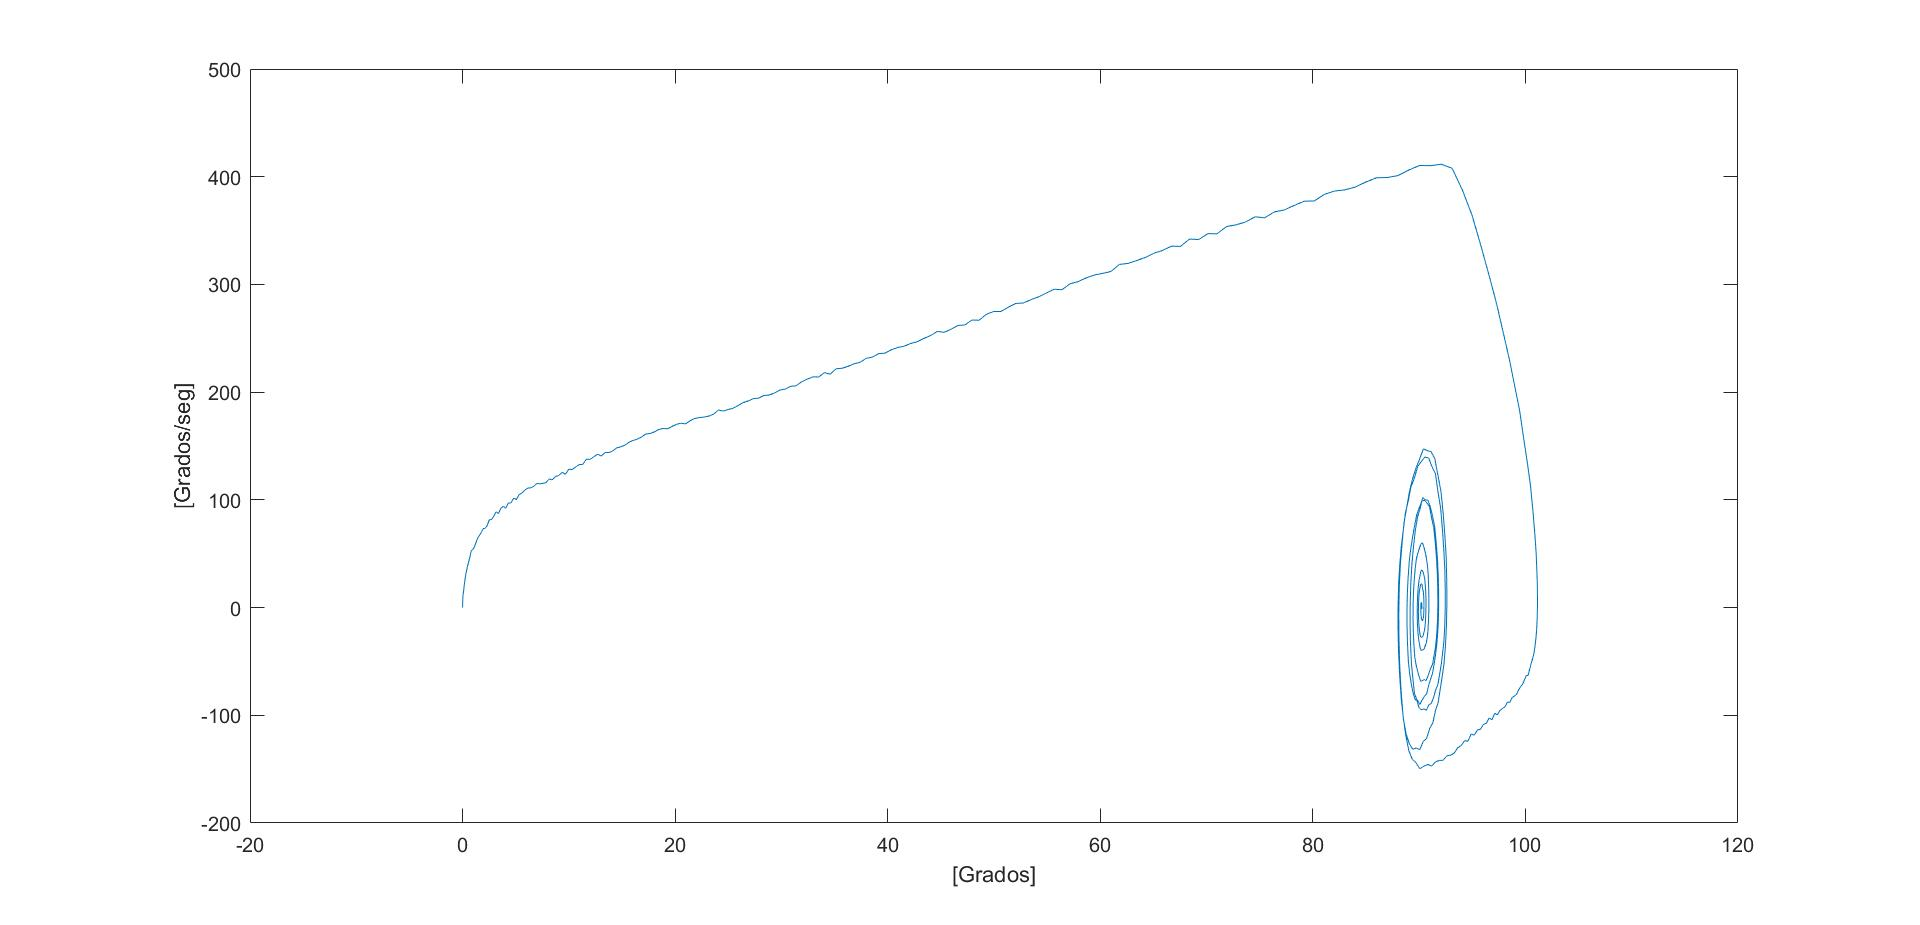
\includegraphics[width=10cm]{IMAGENES/1}
        \caption{Espectro de una señal Muestreada.}
        \label{fig:espectro}
\end{figure}

Las repeticiones del espectro en la figura \ref{fig:espectro} no deben solaparse para evitar la superposición de frecuencias, para evitar este problema el teorema de Nyquist nos dice que se debe cumplir lo siguiente.

\begin{equation}
    \begin{split}
        |\omega_s-B|>B\to \omega_s>2B\\
    \end{split}
    \label{eq:espectro_muestreada}
\end{equation}

Esta desigualdad se conoce como la frecuencia de Nyquist o Shanon, nos garantizará que la señal original se podrá reconstruir apartir de las muestras tomadas.
\subsection{Ejemplo}
Se muestreará una señal senoidal usando matlab.
\lstinputlisting[language=Matlab]{Matlab/finale.m}

\begin{figure}[h]
    \centering
        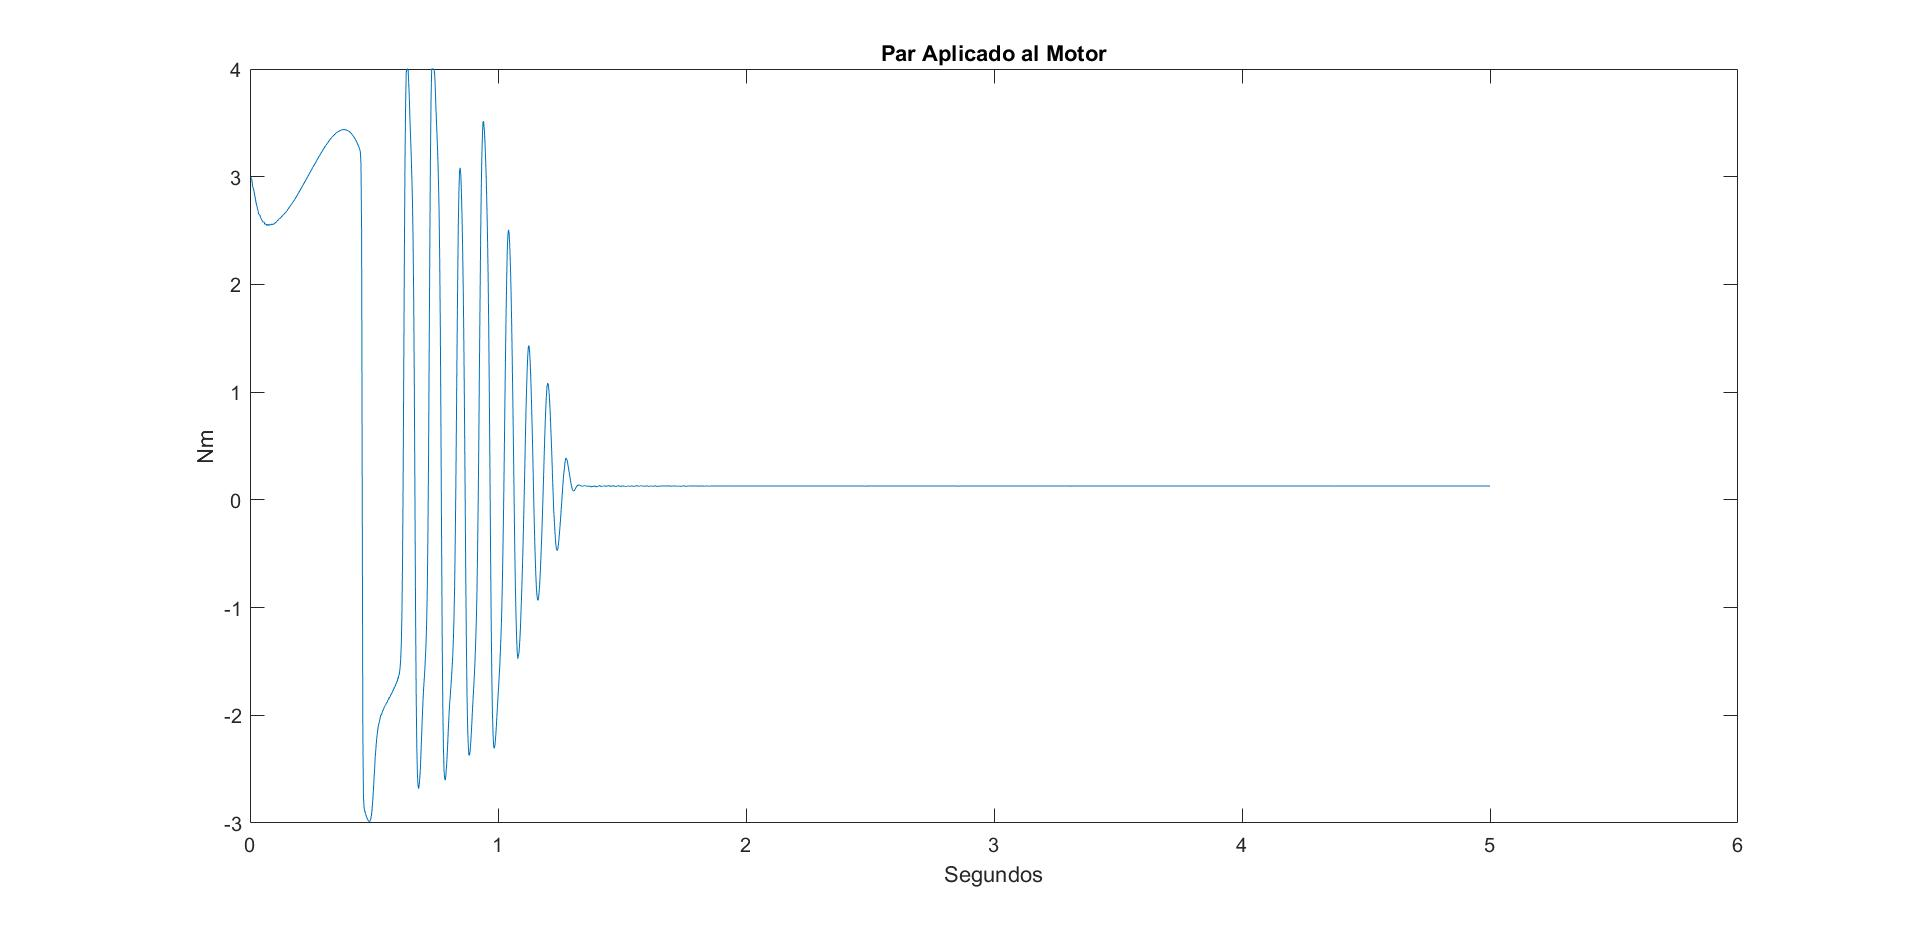
\includegraphics[width=10cm]{IMAGENES/2}
        \caption{Muestreo de señal Senoidal.}
\end{figure}
\section{Transformada de Fourier}
Es un caso especial de la transformada bilateral de Laplace esta se define de la siguiente manera [\cite{lago1984teoria}].

\begin{equation}
    \begin{split}
        F(s)&=\int _{-\infty}^{\infty} e^{-st}f(t)dt\\
    \end{split}
    \label{eq:bilate_laplace}
\end{equation}

Dentro de todo el plano complejo $s$ la transformada de Fourier estará definida para $s=j\omega$ 

\begin{equation}
    \begin{split}
        \mathscr{F}\{f(t)\}=F(\omega)&=\int _{-\infty}^{\infty} e^{-j\omega t}f(t)dt\\
    \end{split}
    \label{eq:fourier_trans}
\end{equation}

\begin{figure}[h]
    \centering
        \includegraphics[width=10cm]{IMAGENES/Diagram1.eps}
        \caption{Plano Complejo S.}
\end{figure}
\subsection{Ejemplo}
Se calculará la transformada de fourier de la función seno, se hara uso del comando "fft" (fast fourier transform), de Matlab.

\lstinputlisting[language=Matlab]{Matlab/finale1.m}

\begin{figure}[h]
    \centering
        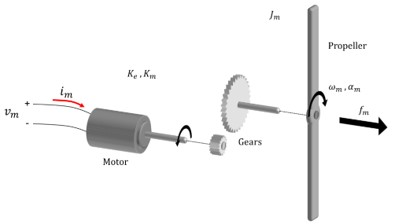
\includegraphics[width=10cm]{IMAGENES/3}
        \caption{Muestreo de señal Senoidal.}
\end{figure}
\vspace{100mm}
\section{Transformada Discreta de Fourier}
En palabras simples es la transformada de fourier en tiempo discreto muestreada, la fórmula se deduce de la siguiente manera.
\\

Sea la transformada unilateral de Laplace
\begin{equation}
    \begin{split}
        X(s)&=\int _{0}^{\infty} e^{-st}x(t)dt\\
    \end{split}
    \label{eq:unila_laplace}
\end{equation}

Usemos esta transformada en la señal muestreada $x(n)=\displaystyle\sum_{n=-\infty}^{\infty}\,x(nT)\delta(t-nT)$

\begin{equation}
    \begin{split}
        X(s)&=\int _{0}^{\infty} \displaystyle\sum_{n=-\infty}^{\infty}\ x(nT)\delta(t-nT)e^{-st}dt\\
        X(s)&=\displaystyle\sum_{n=-\infty}^{\infty}\ x(nT)\int _{0}^{\infty}\delta(t-nT)e^{-st}dt\\ 
        z&=e^{sT}\\
        X(z)&=\displaystyle\sum_{n=-\infty}^{\infty}\ x(nT)z^{-nT}\\
        X(nT)&=X(n)\\
        X(z)&=\displaystyle\sum_{n=-\infty}^{\infty}\ x(n)z^{-n}\\    
    \end{split}
    \label{eq:z_trans}
\end{equation}
La expresión \ref{eq:z_trans} es conocida como la transformada Z. Por la identidad de Euler, sabemos que $e^{j\omega}=cos(\omega)+jsen(\omega)$ tenemos que el periodo de esta expresión es $2\pi$

\begin{figure}[h]
    \centering
        \includegraphics[width=10cm]{IMAGENES/zplane.eps}
        \caption{Plano Complejo Z.}
\end{figure}

Tomando $z=e^{j\omega}$ en \ref{eq:z_trans} se tendrá:

\begin{equation}
    \begin{split}
        X(z)&=\displaystyle\sum_{n=-\infty}^{\infty}\ x(n)e^{-j\omega n}\\    
    \end{split}
    \label{eq:dtft}
\end{equation}

Esta ultima expresión se le conoce como transformada de Fourier en tiempo discreto, en \ref{eq:dtft} se tendrá $\omega=\frac{2\pi k}{N}$ donde es el número de muestras a cuantizar 
\vspace{30mm}
\begin{figure}[h]
    \centering
        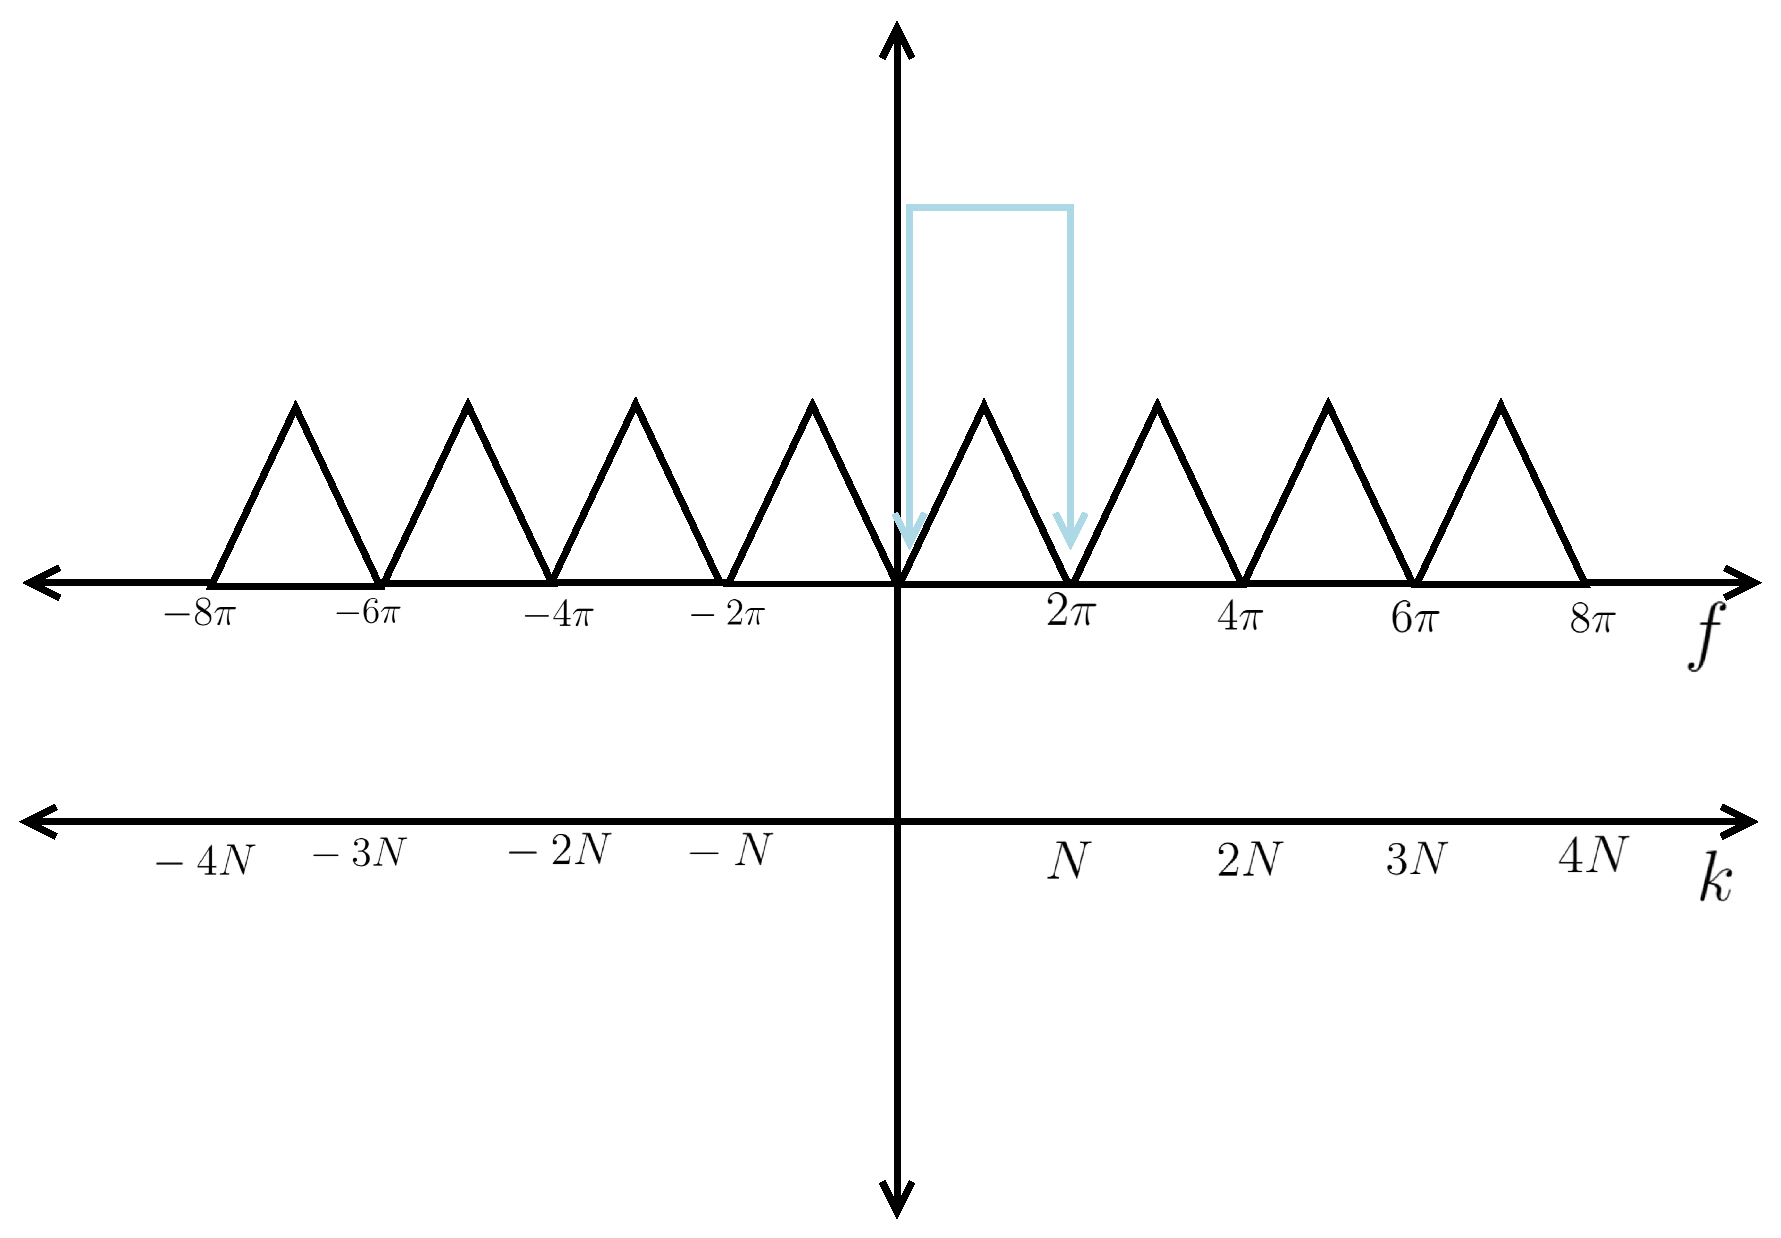
\includegraphics[width=10cm]{IMAGENES/dtft.eps}
        \caption{Muestreo de DFTF.}
\end{figure}


En la figura se puede observar que como $e^{j\omega}$ es periodico solo será necesario tomar un intervalo, haciendo esto, se tendrá.

\begin{equation}
    \begin{split}
        X(\omega)&=X(e^{j\omega})\\
        X(\omega)|_{w=\frac{2\pi k}{N}}&=X(\frac{2\pi k}{N})=...+\displaystyle\sum_{n=-N}^{-1}\ x(n)e^{-j\frac{2\pi kn}{N}}+\displaystyle\sum_{n=0}^{N-1}\ x(n)e^{-j\frac{2\pi kn}{N}}+\displaystyle\sum_{n=N}^{2N-1}\ x(n)e^{-j\frac{2\pi kn}{N}}+...\\
        X(\omega)&=\displaystyle\sum_{n=0}^{N-1}\ x(n)e^{-j\frac{2\pi kn}{N}}\\    
    \end{split}
    \label{eq:dft}
\end{equation}

A la expresión \ref{eq:dft} se le conoce como transformada discreta de fourier.
\subsection{Ejemplo}

Hallar la DFT de la siguiente secuencia $x(n)=\lbrack 1,2,1,0\rbrack$. Usando la definición de DFT se tendrá.
\begin{equation}
    \begin{split}
        k&=0\to X_t\lbrack0\rbrack=1+2+1+0=4\\
        k&=1\to X_t\lbrack1\rbrack=1+e^{\frac{-j\pi}{2}}+e^{\frac{-j\pi}{1}}=-2j\\
        k&=2\to X_t\lbrack2\rbrack=1+2e^{\frac{-j\pi}{1}}+e^{\frac{-j2\pi}{2}}=0\\
        k&=3\to X_t\lbrack3\rbrack=1+2e^{\frac{-j3\pi}{1}}+e^{\frac{-j3\pi}{1}}=2j\\
        X_t\lbrack k\rbrack&=\lbrack4,-2j,0,2j \rbrack\\
    \end{split}
    \label{eq:example_dft}
\end{equation}

\section{Convolución Circular}
La convolución circular de 2 secuencias $x_1(n)$ y $x_2(n)$ esta definida como

\begin{equation}
    \begin{split}
        x(m)&=\displaystyle\sum_{n=0}^{N-1}\ x_1(n)x_2(m-n)\\    
    \end{split}
    \label{eq:circular}
\end{equation}

En el contexto de la transformada discreta de Fourier, la convolución circular en el dominio del tiempo corresponde a la multiplicación las transformadas discretas de cada secuencia.

\begin{equation}
    \begin{split}
        x_1(n)\circledast x_2(n)\to \frac{1}{N}X_1(k)X_2(k)\\    
    \end{split}
    \label{eq:circular}
\end{equation}
\subsection{Ejemplo}
Calcular la convolución circular de las secuencias $x(n)=\lbrack 1,2,1,1\rbrack$ y $h(n)=\lbrack 1,1,-1,-1\rbrack$
Usando la definición se tendrá.
\begin{equation}
    \begin{split}
        x(n)\circledast h(n)\lbrack0\rbrack&=1-2=-1\\
        x(n)\circledast h(n)\lbrack1\rbrack&=2+1-2=1\\
        x(n)\circledast h(n)\lbrack2\rbrack&=1+2-1-1=1\\
        x(n)\circledast h(n)\lbrack3\rbrack&=1+1-2-1=-1\\
        x(n)\circledast h(n)\lbrack n\rbrack&=\lbrack-1,1,1,-1 \rbrack\\
    \end{split}
    \label{eq:example_dft}
\end{equation}
\bibliographystyle{apacite}
\bibliography{biblio}
\end{document}